%
%
\documentclass[a4paper, 11pt]{article}
%
%----------------------------
%---------PACKAGES-----------
%----------------------------
%
%---------geometry
\usepackage{geometry} 
\geometry{margin=2.8cm}
%
%---------spanish
%\usepackage[latin1]{inputenc}
%\usepackage[spanish, es-tabla]{babel}
%
%
%---------version
\usepackage{mversion}
\setVersion{1}
\increaseBuild
%
%---------others
\usepackage{booktabs}
%\usepackage{epigraph} %Epigrafes 
\usepackage{eurosym} %euro symbol
\usepackage[hyphens]{url}
\usepackage{pdfpages} %para incluir pdf como anejos
\usepackage{natbib} %references
\usepackage{array} %math arrays
\usepackage{fancyhdr}
\usepackage{authblk} %affiliations
%
%-----------titles
\usepackage{titlesec}
%\titleclass{\part}{top}
%\titleformat{\part}[hang]{\normalfont\huge\bfseries}{PART \thepart:}{20pt}{\huge }
%\titlespacing*{\part}{0pt}{10pt}{20pt}
%\titleclass{\chapter}{straight}
%\titleformat{\chapter}[hang]{\bf\LARGE}{\thechapter}{2pc}{}
%\titlespacing*{\chapter} {0pt}{20pt}{10pt}
%\titlespacing*{\section} {0pt}{10pt}{10pt}
%
%
%
%---------figures
\usepackage{graphics}
\usepackage{graphicx}
\usepackage{wrapfig} % Allows in-line images ?
\usepackage{color}
\usepackage{amsmath}
\usepackage{amssymb}
%\usepackage{subfigure}
%\usepackage[section]{placeins}
\usepackage[section,subsection,subsubsection]{extraplaceins}
%
%
%---------external references
\usepackage{xr}
%\externaldocument{chapterI}
%
%
%---------tables
\usepackage{multirow} %columns spaning multiple rows
\usepackage{multicol} %rows spaning multiple columns
%
%
%---------minitoc for table of content in every chapter
%\usepackage{minitoc} 
%\ProvidesFile{spanish.mld}[1999/03/16]
%% Spanish titles for minitoc.sty
%\def\mtctitle{\'Indice General}%	
%\def\mlftitle{\'Indice de Figuras}%
%\def\mlttitle{\'Indice de Tablas}%
%\def\ptctitle{\'Indice General}%
%\def\plftitle{\'Indice de Figuras}%
%\def\plttitle{\'Indice de Tablas}%
%\def\stctitle{\'Indice General}%
%\def\slftitle{\'Indice de Figuras}%
%\def\slttitle{\'Indice de Tablas}%
%
%
%
%----------------------------
%---------NEW COMMANDS
%----------------------------
%
%\newcommand{\HRule}{\rule{\linewidth}{0.5mm}}
%\addto\captionsspanish{\renewcommand{\chaptername}{}}
\newcommand{\pathfile}[1]{$<$#1$>$}
\newcommand{\pathdir}[1]{$<$\textbackslash#1\textbackslash$>$}


\setlength{\parindent}{16pt}
\newcommand{\pa}[2]{\ensuremath{\frac{\partial #1}{\partial #2}}}
\newcommand{\paa}[2]{\ensuremath{\frac{\partial^2 #1}{\partial #2^2}}}
\newcommand{\paaa}[2]{\ensuremath{\frac{\partial^3 #1}{\partial #2^3}}}
\newcommand{\paaaa}[2]{\ensuremath{\frac{\partial^4 #1}{\partial #2^4}}}
%
%
%
%----------------------------
%---------PATHS
%----------------------------
%
%\graphicspath{{C:/Users/Victor/Dropbox/PFC/vial_alguaire/proyecto/imagenes/}} %TOSH
%\graphicspath{{D:/victorchavarri/Dropbox/PFC/vial_alguaire/proyecto/imagenes/}} %TUD
%
%
%
%----------------------------
%---------HEADER
%----------------------------
%
\pagestyle{fancy}
\fancyhead[L]{\small ELV}
\fancyhead[R]{\small Model Manual}

%
%
%
%----------------------------
%---------TITLE
%----------------------------
%
\title{
\null
\vfill
\begin{flushright}
\huge{ELV}\\
\vspace{5mm}
\Large{User Manual \& Technical Reference}\\
\vspace{5mm}
\normalsize{\ttfamily{Version: \version}}\\
\vspace{5mm}
%\normalsize{ 
%\begin{tabular}{lr} %anyadir \quad a la formula mas larga
    %Author:    	& V. Chavarr\'ias\\
    %somebody:   & that person\\
%\end{tabular}
 %}
\end{flushright}
}
\date{\today}
\author[1]{V\'ictor Chavarr\'ias}
\author[1]{Liselot Arkesteijn}
\affil[1]{Delft University of Technology}

%--------------------------------------------------------------------------
%
\begin{document}

%
%
%----------------------------
%---------COVER
%----------------------------
%
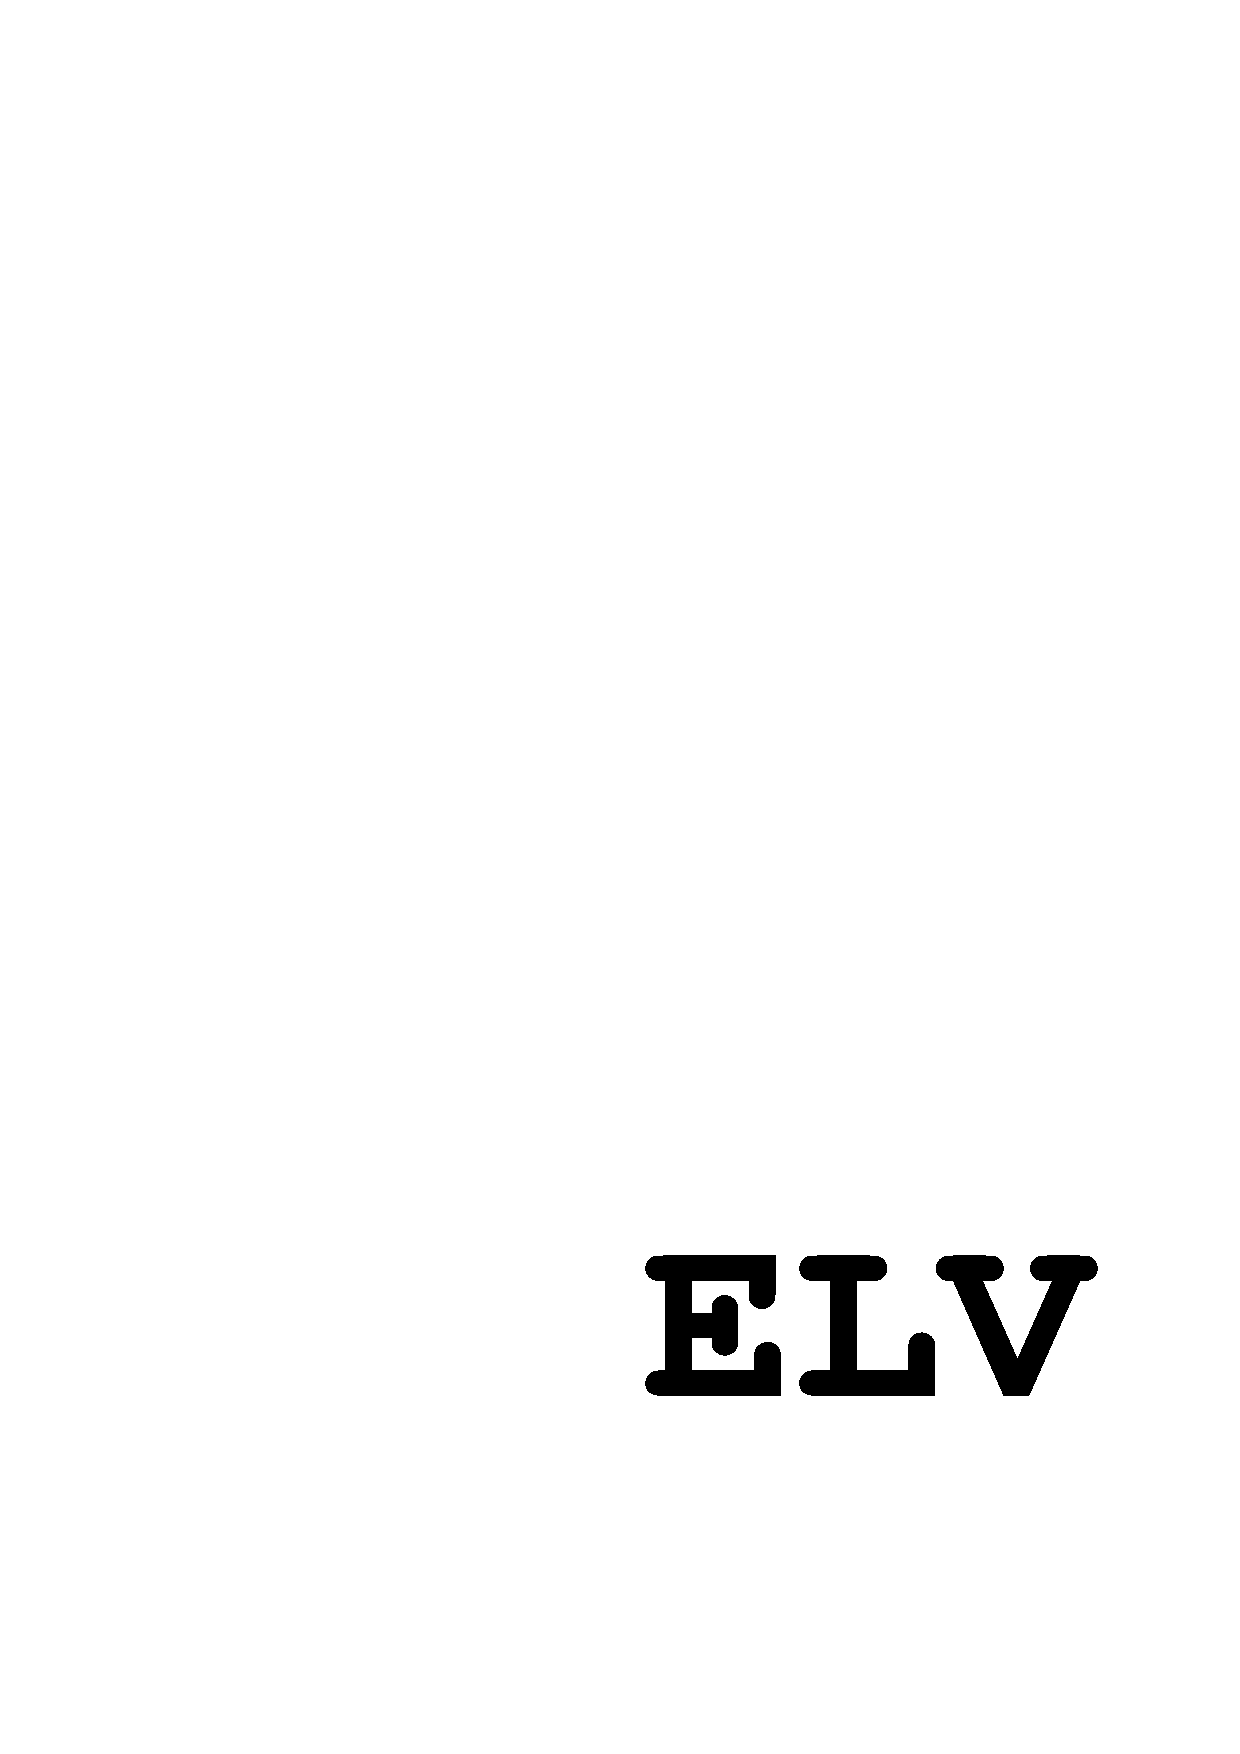
\includepdf{cover.pdf}
\clearpage %for not having number page in the first page
\maketitle
\thispagestyle{empty} %for not having number page in the first page
\pagebreak
\tableofcontents
\clearpage
\pagebreak
%
%
%----------------------------
%---------
%----------------------------
%
%
%
%----------------------------
%---------INTRODUCTION
%----------------------------
%
%\frontmatter
\section*{Preface}
%
ELV is a 1D morphodynamic model, written in Matlab and used as a research model. The model is constructed in a modular way, where the hydrodynamic and morphodynamic behaviour of a 1D single branch river system are solved in a decoupled fashion. This document explains how the model ELV is organized and how to run it. At the end of this manual a tutorial for a first run will be included in the future. Many thanks to the amazing V for creating the structure of ELV and his determination to keep it organized.
\clearpage


%----------------------------
%--------- PART 1: Model structure
%----------------------------
%
\section{Model organization}
\subsection{Introduction}
\subsubsection{Typographical Conventions}
%
Directory names are expressed in between angle brackets and with the backslashes (e.g.\ \pathdir{directory}).

File names in between angle brackets (e.g.\ \pathfile{filename.ext}).

Variables in the model are written in Courier New (e.g.\ \texttt{variable}).

Units are written between vertical brackets (e.g.\ [$m$]).

The kind of variable is written in between vertical brackets and in Courier New font. The size may be specified as a product (e.g.\ [100x1 \texttt{double}])

\subsubsection{Directories Organization}
%
The model is composed of several functions stored in one folder. The folder name is irrelevant, we use \pathdir{ELV}.

A specific run needs a folder. All the input and output files will be stored in this folder. The folder name is irrelevant, e.g.\ \pathdir{r01}. 

The relative location of the folders is irrelevant.

The user may use his/her own working folder with auxiliary scripts, e.g.\ \pathdir{code}.


\subsection{Model layout}
We need to add a nice flowchart; 

%
%----------------------------
%---------
%----------------------------
%

\subsection{SVN version control}
To be updated by the amazing V;
%
%
%----------------------------
%---------
%----------------------------
%

\clearpage



































%
%
%----------------------------
%---------PART 2: EQUATIONS
%----------------------------
%
\clearpage
\section{Governing equations}
\subsection{Flow model}
\subsubsection{Saint-Venant}
For the unsteady flow solver; the 1D Saint-Venant equations are solved. ADD MORE ONCE WIDTH VARIATIONS ARE INCLUDED

\subsubsection{Diffusive wave model}

\subsubsection{Backwater model}
At the moment two implementations of the backwater model are present, one using the conservation of energy, the other starting from momentum conservation. The latter implementation accounts for compound channels.
\subsubsection*{Solver 1}
 The first solver uses the energy conservation principle.

\begin{eqnarray}
H &=& \eta + h + \frac{u^2}{2g}\\
S_f &=& \frac{c_f u^2}{gh}\\
\frac{\partial H}{\partial s} &=& -S_f
\end{eqnarray}

The solution procedure is as follows:
\begin{enumerate}
\item Compute the specific discharge at each location
\item Compute the downstream energy, based on the downstream boundary condition and local specific discharge;
\item Compute the friction slope
\item March upstream using an Euler forward method
\end{enumerate}
All variables are computed at the cell's centers.

\subsubsection*{Solver 2}
See Appendix B for details;


\subsection{Sediment mass conservation model}
\subsubsection{Exner}
\subsubsection{Hirano}
Add some details on the substrate?

\subsection{Equilibrium models}
\subsubsection{Analytical model}
\subsubsection{Space-marching model}

\clearpage












































\section{Model setup}

\subsection{Workflow}
%
%

\begin{enumerate}
\item The user creates the simulation directory (e.g.\ \pathdir{r01}). 
\item The user creates a Matlab variable called \pathfile{input.mat} containing the input for the simulation in that folder.
\item The user calls the function \pathfile{run\_ELV.m} in which the argument is \pathfile{input.mat}.
\item The simulation runs and the results are stored in \pathfile{input.mat} in the same folder.
\item The postprocessing runs and the figures are stored under a folder called \pathdir{r01\textbackslash figures}.
\end{enumerate}

How to input is explained in Section \ref{sec:input}. The run process is explained in Section \ref{sec:run}. The model itself is explained in Section \ref{sec:elv}.


%
%
%----------------------------
%---------
%----------------------------
%
\subsection{Run}
%
\label{sec:run}
%
Once the input file is created, to run a simulation the user needs to call the function \pathfile{run\_ELV} (Appendix \ref{app:run_ELV}). This consist of:
\begin{enumerate}
\item Initialization \pathdir{output} and \pathdir{figures}.
\item Call to the main function \pathfile{ELV} (Section \ref{sec:elv}).
\item Call to the postprocessing routines. 
\end{enumerate}

%
%----------------------------
\subsubsection{Initialization}
%----------------------------
\label{subsec:run_ini}

In this part the folder where the figures are going to be written are created and the log file is created.

%
%----------------------------
\subsubsection{Call to ELV}
%----------------------------
\label{subsec:run_elv}

In this part the main function is called.

%
%----------------------------
\subsubsection{Postprocessing}
%----------------------------
\label{subsec:run_post}

In this part the postprocessing routines are called. 




%
%
%
%----------------------------
%---------
%----------------------------
%
\subsection{ELV}
%
\label{sec:elv}
%
The mathematically dependent variables of the model are $u$, $h$, $\eta_b$, and $M_{ak}$:
\begin{itemize}
\item \texttt{u   }: mean flow velocity [$m/s$]; [1x$n_x$ \texttt{double}]
\item \texttt{h   }: flow depth [$m$]; [1x$n_x$ \texttt{double}]
\item \texttt{etab}: bed elevation [$m$]; [1x$n_x$ \texttt{double}]
\item \texttt{Mak }: sediment mass in the active layer per unit area [$m$]; [$n_f$x$n_x$ \texttt{double}]
\end{itemize}

Other variables in the model are:
\begin{itemize}
\item \texttt{qbk  }: specific sediment transport per grain size excluding pores [$m^2/s$]; [$n_f$x$n_x$ \texttt{double}]
\item \texttt{Cf   }: dimensionless friction coefficient [$-$]; [1x$n_x$ \texttt{double}]
\item \texttt{La   }: active layer thickness [$m$]; [1x$n_x$ \texttt{double}]
\item \texttt{Msk  }: sediment mass in the substrate per unit area [$m$]; [$n_f$x$n_x$x$n_{sl}$ \texttt{double}]
\end{itemize}

All the variables are organized as follows:
\begin{itemize}
\item in dimension 1 (row) they store the data per size fraction ($k$). 
\item in dimension 2 (colums) they store the data streamwise direction ($x$).
\item in dimension 3 they store the data per layer (only the substrate data) ($sl$).
\end{itemize}

The main function is called \pathfile{ELV} (Appendix \ref{app:ELV}). This function contains the following parts:
\begin{enumerate}
\item Initialization (Section \ref{subsec:elv_ini})
\item Preprocessing (Section \ref{subsec:elv_pre})
\item Time Loop (Section \ref{subsec:elv_time})
\end{enumerate}



\subsection{Equilibrium models}
ELV contains a special option to compute the equilibrium state of the river under the prescribed boundary conditions. There are three options for this, each of which are accesible within ELV and as a seperate model funtion. 

\subsubsection{Equilibrium with ELV}
The equilibrium state using a time-marching model within ELV is found by setting the total simulation time of the run to NaN. The remainder of the workflow stays the same. An automatic criterion for equilibrium is implemented, based on the periodicity of the external forcings.  

\subsubsection{Normal flow analytical equilibrium solution}
The equilibrium state in the normal flow segment, as described by the analytical equilibrium solution can be found using the same workflow as for ELV, but rather than that calling the function \pathfile{run\_nfanalyt.m} in which the argument is \pathfile{input.mat}. The variable \pathfile{input.mat} can be specified the same as in ELV, however, not all variables needed for a transient simulation are needed here aswell.

\subsubsection{Space-marching solution}
The equilibrium state computed using a space marching procedure can be obtained by running \pathfile{run\_spacemarching.m}, rather than \pathfile{run\_nfanalyt.m}. This is one opition, in addition when a transient simulation is started from a space-marching equilibrium solution, the entire workspace after space-marching is stored in  \pathfile{output\_sp.mat}.





































































































































%
%
%----------------------------
%--------- PART III: INPUT Specification
%----------------------------
%
%
%

%
\clearpage
\section{Input parameter specification in \pathfile{input.mat}} 
%
\label{sec:input}
%
%----------------------------
%\subsection{Creation of \pathfile{input.mat}}
%----------------------------
%\label{subsec:input_creation}
%
There are 2 ways of creating the variable called \pathfile{input.mat}: 
\begin{enumerate}
\item Via script
\item Via ascii-files 
\end{enumerate}

For option 1 we provide the script \pathfile{input\_single\_ELV.m}. The values are written in the script and when executed the variable is created in the target folder. Similar scripts can be used to automatically generate several simulations.

For option 2 we provide the script \pathfile{input\_dir\_ELV.m}. The input is the folder containing the ascii-files. The files can be either the input files of the old model or Delft3D input files.
%
%----------------------------
%\chapter{Structure of \pathfile{input.mat}}
%----------------------------
\label{subsec:input_structure}
%
\pathfile{input.mat} contains one single variable called \texttt{input}. The variable input is a structure array that contains
\begin{itemize}
\item \texttt{input.run}: run identificator [\texttt{char}]
\item \texttt{input.mdv}: master definition variables [\texttt{struct}]
\item \texttt{input.grd}: grid [\texttt{struct}]
\item \texttt{input.mor}: morphology [\texttt{struct}]
\item \texttt{input.sed}: sediment characteristics [\texttt{struct}]
\item \texttt{input.tra}: sediment transport [\texttt{struct}]
\item \texttt{input.ini}: initial condition [\texttt{struct}]
\item \texttt{input.bch}: hydrodynamic boundary conditions [\texttt{struct}]
\item \texttt{input.bcm}: morphodynamic boundary conditions [\texttt{struct}]
\item \texttt{input.nour}: variables related to including a nourishment [\texttt{struct}]
\item \texttt{input.oth}: remaining variables or conditions, waiting to be categorized at a later stage [\texttt{struct}]
\end{itemize}

In this section we will use the following notation:
\begin{itemize}
\item $n_f$ stands for the number of sediment size fractions.
\item $n_x$ stands for the number of nodes in streamwise direction. 
\item $n_{sl}$ stands for the number of substrate layers.
\item $n_i$ stands for the number of input values.
\end{itemize}
%
%\chapter{Run specification and flow module settings}
\subsection{Run Identificator (\texttt{input.run})}
\label{subsubsec:in_run}
%
\texttt{input.run} contains the tag that identifies a run.
\begin{itemize}
\item \texttt{input.run}: simulation name [\texttt{char}]; e.g.\ \texttt{'L\_05'}
\end{itemize}
%
\subsection{Master Definition (\texttt{input.mdv})}
\label{subsubsec:in_mdv}
%
\texttt{input.mdv} contains the general variables and flags of the run.
\begin{itemize}
\item \texttt{input.mdv.flowtype    }: flow assumption: 1=steady; 2=quasi-steady; 3=unsteady explicit; 4 = unsteady implicit (Preismann); 5 = space-marching model [1x1 \texttt{double}]; e.g.\ [1]
\item \texttt{input.mdv.fluxtype    }: fluxtupe in case of unsteady explicit method: 1=..; 2=..; 3=...; [1x1 \texttt{double}]; e.g.\ [1]
\item \texttt{input.mdv.frictiontype}: friction type: 1=constant; 2=related to grain size; 3=related to flow depth; [1x1 double]; e.g. [1]
\item \texttt{input.mdv.Tstop       }: simulation time [$s$]; [1x1 \texttt{double}]; e.g.\ [3600]. When NaN is specified as input, the simulation is ran until equilibrium is reached. 
\item \texttt{input.mdv.dt          }: time step [$s$]; [1x1 \texttt{double}]; e.g.\ [2]
\item \texttt{input.mdv.Flmap\_dt   }: printing map-file interval time [$s$]; [1x1 \texttt{double}]; e.g.\ [60]   
\item \texttt{input.mdv.Cf          }: friction coefficient [$-$]; [1x1 \texttt{double}]; e.g.\ [0.008]
\item \texttt{input.mdv.rhow        }: water density [$kg/m^3$]; [1x1 \texttt{double}]; e.g.\ [1000]
\item \texttt{input.mdv.g           }: gravity constant [$m/s^2$]; [1x1 \texttt{double}]; e.g.\ [9.81]
\end{itemize}
When the friction is [1x1 \texttt{double}], or  a vector [1x$n_x$ \texttt{double}], then the cross-section is rectangular. For the latter, rather than the same value along the entire domain the vector specifies the value per node. For the space-marching method the friction is interpolated.  In the solver-option of flowtype 6, it is possible to specify a non-rectangular cross-section. The input should then be specified as [4x1 \texttt{double}] (constant along the streamwise) or   [4x$n_x$ \texttt{double}], varying within the cross-section and per node. The rows are respectively 1) representative friction (NaN); 2) main channel friction; 3) left flood plain friction; and 4) right flood plain friction.

%
%
\subsection{Grid (\texttt{input.grd})}
\label{subsubsec:in_grd}
%
\texttt{input.grd} contains the general variables and flags of the run.
\begin{itemize}
\item \texttt{input.grd.L }: domain length [$m$]; [1x1 \texttt{double}]; e.g.\ [100]
\item \texttt{input.grd.B }: domain width [$m$]; [1x1 \texttt{double}]; e.g.\ [1]
\item \texttt{input.grd.dx}: streamwise discretizations [$m$]; [1x1 \texttt{double}]; e.g.\ [0.1]
\end{itemize}
%
When the width is [1x1 \texttt{double}], or  a vector [1x$n_x$ \texttt{double}], then the cross-section is rectangular. For the latter, rather than the same value along the entire domain the vector specifies the value per node. For the space-marching method the width is interpolated.  In the solver-option of flowtype 6, it is possible to specify a non-rectangular cross-section. The input should then be specified as [4x1 \texttt{double}] (constant cross-section) or   [4x$n_x$ \texttt{double}], cross-section per node. The rows are respectively 1) total width; 2) main channel width; 3) left flood plain width; and 4) right flood plain width.


\subsection{Morphology (\texttt{input.mor})}
\label{subsubsec:in_mor}
%
%
$input.mor$ contains the morphology input.
\begin{itemize}
\item \texttt{input.mor.bedupdate        }: flag to update the bed: 0=No; 1=Yes [$-$]; [1x1 \texttt{double}]; e.g.\ [1]
\item \texttt{input.mor.gsdupdate        }: flag to update the grain size distribution: 0=No; 1=Yes [$-$]; [1x1 \texttt{double}]; e.g.\ [1]
\item \texttt{input.mor.ellcheck        }: flag to check for ellipticity: 0=No; 1=Yes [$-$]; [1x1 \texttt{double}]; e.g.\ [1]
\item \texttt{input.mor.Latype        }: active layer assumption: 1=constant thickness; 2=linked to grain size; 3=linked to flow depth; [1x1 \texttt{double}]; e.g.\ [1]
\item \texttt{input.mor.La            }: active layer thickness [$m$]; [1x1 \texttt{double}]; e.g.\ [0.1]
\item \texttt{input.mor.ThUnLyr       }: thickness of each underlayer [$m$]; [1x1 \texttt{double}]; e.g.\ [0.15]
\item \texttt{input.mor.interfacetype    }: fractions at the interface 1=Hirano; 2=Hoey and Ferguson [-]; [1x1 \texttt{double}]; e.g.\ [1]
%\item \texttt{input.mor.ThFnLyr       }: thickness of the final substrate layer [$m$]; [1x1 \texttt{double}]; e.g.\ [0.15]
\item \texttt{input.mor.total\_ThUnLyr}: thickness of the entire bed [$m$]; [1x1 \texttt{double}]; e.g.\ [2]
\item \texttt{input.mor.MorStt        }: spin-up time [$s$]; [1x1 \texttt{double}]; e.g.\ [60]
\item \texttt{input.mor.MorFac        }: morphological accelerator factor [$-$]; [1x1 \texttt{double}]; e.g.\ [10]
\item \texttt{input.mor.porosity	}: bed porosity [-]; [1x1 double]; e.g. [0.4]
\end{itemize}

%\item \texttt{input.mor.ThFnLyr}
%
\subsection{Sediment Characteristics (\texttt{input.sed})}
\label{subsubsec:in_sed}
%
%
\texttt{input.sed} contains the sediment characteristics.
\begin{itemize}
\item \texttt{input.sed.dk  }: characteristic grain sizes [$m$]; [$n_f$x1 \texttt{double}]; e.g.\ [0.0005;0.003;0.005]
\item \texttt{input.sed.rhos}: sediment density [$kg/m^3$]; [1x1 \texttt{double}]; e.g.\ [2650]
\end{itemize}
%
\subsection{Sediment Transport (\texttt{input.tra})}
\label{subsubsec:in_tra}
%
\texttt{input.tra} contains the sediment transport input.
\begin{itemize}
\item \texttt{input.tra.cr   }: sediment transport closure relation: 1=Meyer-Peter-M\"uller; 2=Engelund-Hansen; 3=Ashida-Michiue; 4=Wilcock-Crowe; 5= Generalized Load relation [1x1 \texttt{double}]; e.g.\ [1]
\item \texttt{input.tra.param}: sediment transport parameters (depending on the closure relation) Default values (to be implemented are:)
\begin{enumerate}
\item MPM: e.g.\ [8, 1.5, 0.047]
\item EH: e.g.\ [0.05, 5] 
\item AM: e.g.\ [17, 0.05]
\item WC, no parameters required
\item GL: e.g. \ [ , ]
\end{enumerate}
\item \texttt{input.tra.hid  }: hiding function: 0=NO function; 1=Egiazaroff; 2=Power-Law; 3=Ashida-Mishihue;
\end{itemize}

%
\subsection{Initial Condition (\texttt{input.ini})}
\label{subsubsec:in_ini}
%
\texttt{input.ini} contains the initial condition.
\begin{itemize}
\item \texttt{input.ini.initype}: kind of initial condition: 1=normal flow equilibrium (given an upstream sediment load); 2=free (manually define); 3 =from file; 4= space-marching equilibrium (given an upstream sediment load) [1x1 \texttt{double}]; e.g.\ [1]
\end{itemize}

If the initial condition is set to be free, input is required for:
\begin{itemize}
\item \texttt{input.ini.u      }: flow velocity [$m/s$]; [1x1 \texttt{double}]; e.g.\ [10]
\item \texttt{input.ini.h      }: flow depth [$m$]; [1x1 \texttt{double}]; e.g.\ [10]
\item \texttt{input.ini.slopeb }: bed slope [$-$]; [1x1 \texttt{double}]; e.g.\ [10]
\item \texttt{input.ini.etab0  }: downstream bed elevation [m]; [1x1 \texttt{double}]; e.g.\ [10]
\item \texttt{input.ini.etab   }: bed elevation [$m$]; [1x1 \texttt{double}]; e.g.\ [10]
\item \texttt{input.ini.Fak    }: effective fractions at the active layer [$-$]; [$(n_f-1)$x1 \texttt{double}]; e.g.\ [0.2,0.3]
\end{itemize}
for all except \texttt{input.ini.etab0  } and \texttt{input.ini.Fak}, the input can also be a vector [1x$n_x$ \texttt{double}]. For \texttt{input.ini.Fak}, the input can also be a matrix with dimensions [$(n_f-1)$x$n_x$x$n_{sl}$ \texttt{double}]. Then, rather than the same value along the entire domain the vector specifies the value per node. 
You can either specify \texttt{input.ini.slopeb} and \texttt{input.ini.etab0} or \texttt{input.ini.etab}. All of them is redundant and throws an error.\\

For the restart from file, a path to another result folder and a time step at which the results should be loaded are required:
\begin{itemize}
\item \texttt{input.ini.rst\_file}: path to the folder (be aware of Linux/Windows)!
\item \texttt{input.ini.rst\_resultstimestep}: result time step with the initial condition [$-$]; [1x1 \texttt{double}], e.g. [70]; if NaN it will be the last one.     
\end{itemize}

For all other cases, necessary input is:
\begin{itemize}
\item \texttt{input.ini.fsk    }: effective fractions at the substrate [$-$]; [$(n_f-1)$x1 \texttt{double}]; e.g.\ [0.2,0.3]
\end{itemize}
the input can also be a matrix [$(n_f-1)$x$n_x$x$n_{sl}$ \texttt{double}]. Then, rather than the same value along the entire domain the matrix specifies the values per node and per layer in the substrate. The input can also be the path to a file containing the full matrix. Also, the input can be a string 'Fak'; which indicates the values of 'Fak' (either via input or automatically computed) are copied.\\

For the space-marching equilibrium, an extra struct input.ini.sp is required, with following fields:
\begin{itemize}
\item \texttt{input.ini.sp.intype }: specification of upstream boundary condition; 1 = hydrograph series (Q,t) , 2=discrete probability distribution (Q,p(Q)) [$-$]; e.g.\ [1]
\item \texttt{input.ini.sp.outtype}: specification of output; 1 = mean variables; 2 = mean bed elevation and dominant discharge flow variables; 3 = first time step variables (suited for periodic bcs); 4 = full output (variables during all discharges)
\item \texttt{input.ini.sp.nmodes}: Number of modes [$-$] to discretize the pdf in (only applicable when no time reconstruction is performed),   e.g.\ [100]
\item \texttt{input.ini.sp.dx}: Space marching step  [$m$]; [1x1 \texttt{double}],  e.g.\ [1]. Overwrites the default automatic guess.
\item \texttt{input.ini.sp.al}: Average annual load, use this as an overwrite to start from a different equilibrium condition.
\end{itemize}



%
\subsection{Hydrodynamic Boundary Conditions (\texttt{input.bch})}
\label{subsubsec:in_bch}
%
\texttt{input.bch} contains the boundary condition for hydraulics.
\begin{itemize}
\item \texttt{input.bch.uptype   }: type of hydrodynamic boundary condition at the upstream end: {1,11}=water discharge from input; 12 = water discharge from matlab file; 13 = daily discharge series from ascii-file; 14 = SOBEK-discharge file [-]; e.g. [1]
\item \texttt{input.bch.dotype   }: type of hydrodynamic boundary condition at the downstream end: {1,11}=water level from input; 12 = water level from file; {2,21}=water depth from input; 22=water depth from file  [-]; [1x1 \texttt{double}]; e.g. [1]\\
\end{itemize}
For the input specification from file; if a too short time series is prescribed, the series automatically repeated until the end of the total simulation time. For the boundary conditions from input this is not the case!

When the boundary conditions are specified from file, they can by default be saved as a time series at the result folder. Otherwise, define:
\begin{itemize}
\item \texttt{input.bch.path\_file\_Q  }: pathname where data is located [-] 
\item \texttt{input.bch.path\_file\_etaw0}: pathname where data is located [-]\\
\end{itemize}
When the variables are declared from input; the following are required:
\begin{itemize}
\item \texttt{input.bch.timeQ0   }: time at which the specific water discharge is specified [$s$]; [$n_i$x1 \texttt{double}]; e.g.\ [1800;3600]
\item \texttt{input.bch.Q0       }: water discharge at the specified times [$m^3/s$]; [$n_t$x1 \texttt{double}]; e.g.\ [1;2]
\item \texttt{input.bch.timeetaw0}: time at which the downstream water level is specified [$s$]; [$n_i$x1 \texttt{double}]; e.g.\ [1800;3600]
\item \texttt{input.bch.etaw0    }: downstream water level at the specified times [$m$]; [$n_t$x1 \texttt{double}]; e.g.\ [1;1.5]
\end{itemize}

%
\subsection{Morphodynamic Boundary Condition (\texttt{input.bcm})}
\label{subsubsec:in_bcm}
%
\texttt{input.bcm} contains the boundary condition for morphology.
\begin{itemize}
\item \texttt{input.bcm.type    }: type of morphodynamic boundary condition: {1,11}=sediment discharge from input; 12 = sediment discharge from file; 13 = normal flow load distribution
\item \texttt{input.bcm.NFLtype }: type of variables specified for normal flow load computation: 1 = slope and active layer bed fractions; 2 = average annual load and bed fractions; 3 = average annual load per fraction 
\item \texttt{input.bcm.NFLparam   }: input parameters
\begin{enumerate}
\item [slope, frac1, frac2, ... fracN]. The fractions should add up to one. For unisize simulations only the slope is required.
\item [AL, frac1,frac2,...,fracN]. The fractions should add up to one. For unisize simulations only the average load is required.
\item [Al1,AL2,...ALN].
\end{enumerate}
\item \texttt{input.bcm.NFLiparam   }: (optional) provide a sophisticated initial guess to have better changes to find the solution
\begin{enumerate}
\item not implemented yet
\item not implemented yet
\item \[AL1,AL2,...ALN \].
\end{enumerate}
\item \texttt{input.bcm.timeQbk0}: time at which the input is specified [$s$]; [$n_i$x1 \texttt{double}]; e.g.\ [1800;3600]
\item \texttt{input.bcm.Qbk0    }: volume of sediment transported excluding pores per unit time, and per size fraction at the specified times [$m^3/s$]; [$n_t$x$n_f$ \texttt{double}]; e.g.\ [2e-4,4e-4;3e-4,5e-4]
\item \texttt{input.bcm.path\_file\_Qbk0}: pathname where data is located [-], default is the result folder.
\end{itemize}

\subsection{Nourishment variables (\texttt{input.nour})}
\label{subsubsec:in_nour}
Add nourishment things



























































%-------------------------------------------------------------------------------------------------------------------------------------------------------------------------------------------
%
%
%	PART 4: FUNCTIONS
%
%


\clearpage
\section{Functions}
\subsection{ELV.m}
ELV is the main function of the model \\ 
 \\ 
ELV(path\_file\_input,fid\_log) \\ 
 \\ 
INPUT: \\ 
   -path\_file\_input = path to the file input.mat; $[$char$]$;  \\ 
	-fid\_log = log file identifier \\ 
 \\ 
OUTPUT: \\ 
   - \\ 
 \\ 
\subsection{ELV\_version.m}
ELV\_version is a function that writes the version of each function in the log file \\ 
 \\ 
ELV\_version(fid\_log) \\ 
 \\ 
INPUT: \\ 
   -fid\_log = file identifier \\ 
 \\ 
OUTPUT: \\ 
   - \\ 
 \\ 
\subsection{active\_layer\_mass\_update.m}
active\_layer\_mass\_update updates the mass (volume) of sediment at the active layer. \\ 
 \\ 
\texttt{Mak\_new=active\_layer\_mass\_update(Mak,detaLa,fIk,qbk,bc,input,fid\_log,kt)} \\ 
 \\ 
INPUT: \\ 
   -\texttt{Mak} = effective volume of sediment per unit of bed area in the active layer $[$m$]$; $[$(nf-1)x(nx) double$]$ \\ 
   -\texttt{detaLa} = variation in elevation of the interface between the active layer and the substarte $[$m$]$; $[$(1)x(nx) double$]$ \\ 
   -\texttt{fIk} = effective volume fraction content of sediment at the interface between the active layer and the substrate $[$-$]$; $[$(nf-1)x(nx) double$]$ \\ 
   -\texttt{qbk} = volume of sediment transported excluding pores per unit time and width and per size fraction $[$m$^2$/s$]$; $[$(nf)x(nx) double$]$ \\ 
   -\texttt{bc} = boundary conditions structure  \\ 
   -\texttt{input} = input structure \\ 
   -\texttt{fid\_log} = identificator of the log file \\ 
   -\texttt{kt} = time step counter $[$-$]$; $[$(1)x(1) double$]$ \\ 
 \\ 
OUTPUT: \\ 
   -\texttt{Mak\_new} = new effective volume of sediment per unit of bed area in the active layer $[$m$]$; $[$(nf-1)x(nx) double$]$ \\ 
 \\ 
\subsection{active\_layer\_mass\_update\_pmm.m}
function\_name does this and that \\ 
 \\ 
Mak\_new=active\_layer\_mass\_update\_pmm(Mak,detaLa,fIk,qbk,bc,pmm,input,fid\_log,kt) \\ 
 \\ 
INPUT: \\ 
   - \\ 
 \\ 
OUTPUT: \\ 
   - \\ 
 \\ 
\subsection{active\_layer\_thickness\_update.m}
active\_layer\_thickness\_update is a function that updates the active layer thickness \\ 
 \\ 
La=active\_layer\_thickness\_update(h,Mak,La\_old,input,fid\_log,kt) \\ 
 \\ 
INPUT: \\ 
   - \\ 
 \\ 
OUTPUT: \\ 
   - \\ 
 \\ 
\subsection{add\_nourishment.m}
add\_nourishment modifies the bed adding nourished sediment \\ 
 \\ 
$[$Mak\_new,msk\_new,Ls\_new,La\_new,etab\_new,h\_new$]$=add\_nourishment(Mak\_old,msk\_old,Ls\_old,La\_old,etab\_old,h\_old,input,fid\_log,kt) \\ 
 \\ 
INPUT: \\ 
   - \\ 
 \\ 
OUTPUT: \\ 
   - \\ 
 \\ 
\subsection{add\_sedflags.m}
add\_sedflags parse the sediment input and adds the sediment transport relation flags to the input structure  \\ 
 \\ 
input=add\_sedflags(input) \\ 
 \\ 
INPUT: \\ 
   -input = input structure \\ 
 \\ 
OUTPUT: \\ 
   -input = input structure \\ 
 \\ 
\subsection{analytical\_cubic\_root.m}
analytical\_cubic\_root returns the three roots of a cubic polynomial, provided they are real. \\ 
 \\ 
root=analytical\_cubic\_root(a\_coeff, b\_coeff, c\_coeff, d\_coeff) \\ 
 \\ 
INPUT: \\ 
   -a\_coeff = a coefficient of the polynomial \\ 
   -b\_coeff = b coefficient of the polynomial \\ 
   -c\_coeff = c coefficient of the polynomial \\ 
   -d\_coeff = d coefficient of the polynomial \\ 
 \\ 
OUTPUT: \\ 
   -root = three roots \\ 
 \\ 
\subsection{aux\_ini\_normalflow.m}
aux\_ini\_normalflow is an auxiliary function that returns the difference between the boundary condition values of q and qbk and the computed ones \\ 
 \\ 
F=aux\_ini\_normalflow(X,objective,flg,cnt,cf,La,dk,sed\_trans\_param,hiding\_param,mor\_fac) \\ 
 \\ 
INPUT: \\ 
   -input = variable containing the input $[$struct$]$ e.g. input \\ 
 \\ 
OUTPUT: \\ 
   -a .bcm compatible with D3D is created in file\_name \\ 
 \\ 
\subsection{aux\_swc.m}
aux\_swc is an auxiliary function of side\_wall\_corection \\ 
 \\ 
F=aux\_swc(X,u,Sf,input) \\ 
 \\ 
INPUT: \\ 
	-X =  \\ 
	-u =  \\ 
	-Sf = \\ 
   -input =  \\ 
 \\ 
OUTPUT: \\ 
   -F =  \\ 
 \\ 
\subsection{backwater.m}
backwater does this and that \\ 
 \\ 
$[$U,H$]$=backwater(ib,Cf,Hdown,Q,input) \\ 
 \\ 
INPUT: \\ 
   -ib = slope vector \\ 
   -Cf = dimensionless representative friction \\ 
   -Q = upstream discharge (constant), or a discharge vector; \\ 
 \\ 
OUTPUT: \\ 
   -U =  \\ 
   -H =  \\ 
 \\ 
\subsection{backwater\_step.m}
backwater\_step computes just one step of the solver u,h,etab,Cf should be single values; \\ 
 \\ 
$[$U,H$]$=backwater\_step(x,h,ib,Cf,Q,input) \\ 
 \\ 
INPUT: \\ 
   - \\ 
 \\ 
OUTPUT: \\ 
   - \\ 
 \\ 
\subsection{bed\_level\_update.m}
bed\_level\_update updates the bed elevation \\ 
 \\ 
etab\_new=bed\_level\_update(etab,qbk,bc,input,fid\_log,kt) \\ 
 \\ 
INPUT: \\ 
   -input = variable containing the input $[$struct$]$ e.g. input \\ 
 \\ 
OUTPUT: \\ 
   - \\ 
 \\ 
\subsection{bed\_level\_update\_pmm.m}
bed\_level\_update\_pmm updates the bed elevationconsidering PMM \\ 
 \\ 
etab\_new=bed\_level\_update\_pmm(etab,qbk,bc,pmm,input,fid\_log,kt) \\ 
 \\ 
INPUT: \\ 
   -input = variable containing the input $[$struct$]$ e.g. input \\ 
 \\ 
OUTPUT: \\ 
   - \\ 
 \\ 
\subsection{beta\_pmm.m}
beta\_pmm computes the value of beta such that the eigenvalues of the modified matrix A have the same value of than in the original system matrix. \\ 
 \\ 
beta\_o=beta\_pmm(A,alpha\_i,fid\_log) \\ 
 \\ 
INPUT: \\ 
   -input = variable containing the input $[$struct$]$ e.g. input \\ 
 \\ 
OUTPUT: \\ 
   - \\ 
 \\ 
\subsection{boundary\_conditions\_construction.m}
boundary\_condition\_construction is a function that interpolates the boundary conditions \\ 
 \\ 
bc=boundary\_conditions\_construction(u,h,Mak,La,Cf,input,fid\_log) \\ 
 \\ 
INPUT: \\ 
   -input = variable containing the input $[$struct$]$ e.g. input \\ 
 \\ 
OUTPUT: \\ 
   -bc = boundary conditions $[$struct$]$  \\ 
 \\ 
\subsection{check\_input.m}
check\_input is a function that checks that the input is enough and makes sense \\ 
 \\ 
input\_out=check\_input(input,path\_file\_input,fid\_log) \\ 
 \\ 
INPUT: \\ 
   -input = variable containing the input $[$struct$]$ e.g. input \\ 
 \\ 
OUTPUT: \\ 
   -input = variable containing the input $[$struct$]$ e.g. input \\ 
 \\ 
\subsection{check\_simulation.m}
check\_simulation does this and that \\ 
 \\ 
check\_simulation(u,h,Mak,Mak\_old,msk,msk\_old,La,La\_old,Ls,Ls\_old,qbk,bc,ell\_idx,celerities,pmm,input,fid\_log,kt) \\ 
 \\ 
INPUT: \\ 
   - \\ 
 \\ 
OUTPUT: \\ 
   - \\ 
 \\ 
\subsection{compare\_results.m}
compare\_results compares 2 output file. 0 means they are the same \\ 
 \\ 
$[$equal\_bol\_t,equal\_bol,dif\_idx,dif\_res,dif\_max$]$=compare\_results(output\_ref,output\_chk,var) \\ 
 \\ 
INPUT: \\ 
   - \\ 
 \\ 
OUTPUT: \\ 
   - \\ 
 \\ 
\subsection{condition\_construction.m}
condition\_construction does this and that \\ 
 \\ 
$[$u,h,etab,Mak,La,msk,Ls,Cf,bc$]$ = condition\_construction (input,fid\_log) \\ 
 \\ 
INPUT: \\ 
   -input = input structure \\ 
   -fid\_log = identificator of the log file \\ 
 \\ 
OUTPUT: \\ 
   - \\ 
 \\ 
\subsection{derivatives.m}
function\_name does this and that \\ 
 \\ 
$[$dqb\_dq,dqbk\_dq,dqb\_dMal,dqbk\_dMal$]$=derivatives(u,h,Cf,La,qbk,Mak,input,fid\_log,kt) \\ 
 \\ 
INPUT: \\ 
   -input = variable containing the input $[$struct$]$ e.g. input \\ 
 \\ 
OUTPUT: \\ 
   - \\ 
 \\ 
\subsection{display\_tloop.m}
display\_tloop is a function that displays in command at the end of every time step \\ 
 \\ 
display\_tloop(time\_loop,input,fid\_log,kt) \\ 
 \\ 
INPUT: \\ 
   -input = variable containing the input $[$struct$]$ e.g. input \\ 
 \\ 
OUTPUT: \\ 
   - \\ 
 \\ 
\subsection{dv\_bouss\_coef.m}
dv\_bouss\_coef does this and that \\ 
 \\ 
$[$a1, a2$]$ = dv\_bouss\_coef(input,x,h) \\ 
 \\ 
INPUT: \\ 
   - \\ 
 \\ 
OUTPUT: \\ 
   - \\ 
 \\ 
\subsection{dv\_cross\_aux.m}
dv\_cross\_aux does this and that \\ 
 \\ 
diff = dv\_cross\_aux(input, x, term) \\ 
 \\ 
INPUT: \\ 
   - \\ 
 \\ 
OUTPUT: \\ 
   - \\ 
 \\ 
\subsection{dv\_cross\_section.m}
dv\_cross\_section compute the coefficient resulting from the derivative of the cross section: \\ 
  dAf/dx = a1*(dh/dx) + a2(h) \\ 
The computation is performed in different parts for the main channel and flood planes seperately. \\ 
 \\ 
$[$a1, a2, I\_a1, I\_a2, II\_a1, II\_a2, III\_a1, III\_a2$]$ = dv\_cross\_section(input,x,hh,variable) \\ 
 \\ 
INPUT: \\ 
   -x = should be a node identifier \\ 
   -h = vector with h(1,x) the location at x! \\ 
 \\ 
OUTPUT: \\ 
   - \\ 
 \\ 
\subsection{eli\_1.m}
eli\_1 does this and that \\ 
 \\ 
La\_new=eli\_1(La,ell\_idx,in\_f,input,fid\_log,kt) \\ 
 \\ 
INPUT: \\ 
   - \\ 
 \\ 
OUTPUT: \\ 
   - \\ 
 \\ 
\subsection{elliptic\_nodes.m}
elliptic\_nodes does this and that \\ 
 \\ 
$[$ell\_idx,out$]$=elliptic\_nodes(u,h,Cf,La,qbk,Mak,fIk,input,fid\_log,kt) \\ 
 \\ 
INPUT: \\ 
   -input = variable containing the input $[$struct$]$ e.g. input \\ 
 \\ 
OUTPUT: \\ 
   - \\ 
 \\ 
\subsection{errorprint.m}
errorprint is a function that prints in the log file the error catched \\ 
 \\ 
errorprint(error\_obj,fid\_log) \\ 
 \\ 
INPUT: \\ 
   -input = variable containing the input $[$struct$]$ e.g. input \\ 
 \\ 
OUTPUT: \\ 
   - \\ 
 \\ 
\subsection{flow\_update.m}
flow\_update updates the flow depth and the mean flow velocity. \\ 
 \\ 
$[$u\_new,h\_new$]$=flow\_update(u,h,etab,Cf,bc,input,fid\_log,kt) \\ 
 \\ 
INPUT: \\ 
   -input = variable containing the input $[$struct$]$ e.g. input \\ 
 \\ 
OUTPUT: \\ 
   - \\ 
 \\ 
\subsection{folders\_creation.m}
folders\_creation is a function that created the folder where output may be stored. \\ 
 \\ 
folders\_creation(path\_file\_input,fid\_log) \\ 
 \\ 
INPUT: \\ 
   - \\ 
 \\ 
OUTPUT: \\ 
   - \\ 
 \\ 
\subsection{friction.m}
friction is a function that computed the dimensionless friction coefficient \\ 
 \\ 
Cf=friction(h,Mak,Cf\_old,input,fid\_log,kt) \\ 
 \\ 
INPUT: \\ 
   - \\ 
 \\ 
OUTPUT: \\ 
   - \\ 
 \\ 
\subsection{friction\_correction.m}
friction\_correction corrects the friction coefficient for wall friction and ripples \\ 
 \\ 
$[$Cf\_b$]$=friction\_correction(u,h,Cf,input,fid\_log,kt) \\ 
 \\ 
INPUT: \\ 
   - \\ 
 \\ 
OUTPUT: \\ 
   - \\ 
 \\ 
\subsection{function\_layout.m}
function\_name does this and that \\ 
 \\ 
\texttt{$[$output$]$=function\_name(input)} \\ 
 \\ 
INPUT: \\ 
   -\texttt{input} = variable containing the input $[$struct$]$ e.g. input \\ 
 \\ 
OUTPUT: \\ 
   -\texttt{output} = variable containing the output $[$struct$]$ e.g. input \\ 
 \\ 
\subsection{get\_analytical\_solution.m}
get\_analytical\_solution does this and that \\ 
 \\ 
get\_analytical\_solution(folder\_run) \\ 
 \\ 
INPUT: \\ 
   - \\ 
 \\ 
OUTPUT: \\ 
   - \\ 
 \\ 
\subsection{get\_bouss\_coef.m}
get\_bouss\_coef does this and that \\ 
 \\ 
alpha\_b = get\_bouss\_coef(input,x,hh) \\ 
 \\ 
INPUT: \\ 
   - \\ 
 \\ 
OUTPUT: \\ 
   - \\ 
 \\ 
\subsection{get\_cross\_section.m}
get\_cross\_section does this and that \\ 
 \\ 
$[$T,I,II,III$]$ = get\_cross\_section(input,x,h,variable) \\ 
 \\ 
INPUT: \\ 
   - \\ 
 \\ 
OUTPUT: \\ 
   - \\ 
 \\ 
\subsection{get\_equislope.m}
get\_equislope does this and that \\ 
 \\ 
S = get\_equislope(Qw,input,AL,Fk,X0) \\ 
 \\ 
INPUT: \\ 
   -input = input structure \\ 
 \\ 
OUTPUT: \\ 
   - \\ 
 \\ 
\subsection{get\_equivals.m}
get\_equivals computes the normal load distribution given a hydrograph and the annual load \\ 
 \\ 
$[$S,Fk$]$ = get\_equivals(Qw,input,AL,sedp,X0) \\ 
 \\ 
INPUT: \\ 
   -input = input structure \\ 
 \\ 
OUTPUT: \\ 
   - \\ 
 \\ 
\subsection{get\_equivals2\_pdf.m}
get\_equivals2\_pdf does this and that \\ 
 \\ 
$[$B,Fk$]$ = get\_equivals2\_pdf(pq,dq,input,AL,sedp,S,X0) \\ 
 \\ 
INPUT: \\ 
   -input = input structure \\ 
 \\ 
OUTPUT: \\ 
   - \\ 
 \\ 
\subsection{get\_equivals\_V.m}
get\_equivals\_V is a slight modification of get\_equivals to not display output \\ 
 \\ 
$[$S0,Fak0,sum\_Fak\_obj,max\_rel\_error$]$ = get\_equivals\_V(Qw,input\_1,AL,sedp\_1) \\ 
 \\ 
INPUT: \\ 
   -input = input structure \\ 
 \\ 
OUTPUT: \\ 
   - \\ 
 \\ 
\subsection{get\_equivals\_pdf.m}
get\_equivals\_pdf does this and that \\ 
 \\ 
$[$S,Fk$]$ = get\_equivals\_pdf(pq,dq,input,AL,sedp,X0) \\ 
 \\ 
INPUT: \\ 
   -input = input structure \\ 
 \\ 
OUTPUT: \\ 
   - \\ 
 \\ 
\subsection{get\_flow\_velocities.m}
get\_flow\_velocities does this and that \\ 
 \\ 
U = get\_flow\_velocities(input,x,Q,h,ib) \\ 
 \\ 
INPUT: \\ 
   - \\ 
 \\ 
OUTPUT: \\ 
   - \\ 
 \\ 
\subsection{get\_rep\_fric.m}
get\_rep\_fric does this and that \\ 
 \\ 
Cf\_rep = get\_rep\_fric(input,x,h) \\ 
 \\ 
INPUT: \\ 
   - \\ 
 \\ 
OUTPUT: \\ 
   - \\ 
 \\ 
\subsection{get\_sedigraph.m}
get\_sedigraph does this and that \\ 
 \\ 
Qb = get\_sedigraph(Qw,input,S,Fk) \\ 
 \\ 
INPUT: \\ 
   -input = input structure \\ 
 \\ 
OUTPUT: \\ 
   - \\ 
 \\ 
\subsection{grain\_size\_distribution\_update.m}
grain\_size\_distribution\_update updates the mass at the active layer and the substrate and the substrate thickness \\ 
 \\ 
$[$Mak\_new,msk\_new,Ls\_new,La\_ne,etab\_new,ell\_idx,out\_en,pmm$]$=grain\_size\_distribution\_update(Mak,msk,Ls,La\_old,La,etab\_old,etab,qbk,bc,u,h,Cf,input,fid\_log,kt) \\ 
 \\ 
INPUT: \\ 
   - \\ 
 \\ 
OUTPUT: \\ 
   - \\ 
 \\ 
\subsection{ini\_Cf.m}
ini\_Cf is a function that creates the initial friction coefficient vector \\ 
 \\ 
Cf=ini\_Cf(input,fid\_log) \\ 
 \\ 
INPUT: \\ 
   -input = variable containing the input $[$struct$]$ e.g. input \\ 
 \\ 
OUTPUT: \\ 
   - \\ 
 \\ 
\subsection{ini\_La.m}
ini\_La this function creates the initial active layer thickness vector \\ 
 \\ 
La=ini\_La(input,fid\_log) \\ 
 \\ 
INPUT: \\ 
   -input = variable containing the input $[$struct$]$ e.g. input \\ 
 \\ 
OUTPUT: \\ 
   - \\ 
 \\ 
\subsection{ini\_msk.m}
ini\_msk is a function that creates the substrate variable \\ 
 \\ 
$[$msk,Ls$]$=ini\_msk(La,input,fid\_log) \\ 
 \\ 
INPUT: \\ 
   -input = variable containing the input $[$struct$]$ e.g. input \\ 
 \\ 
OUTPUT: \\ 
   - \\ 
 \\ 
\subsection{ini\_normalflow.m}
ini\_normalflow is a function that finds the normal flow conditions at the first time step.  \\ 
 \\ 
$[$u,h,slopeb,Fak$]$=ini\_normalflow(input,Cf,fid\_log) \\ 
 \\ 
INPUT: \\ 
   -input = variable containing the input $[$struct$]$ e.g. input \\ 
 \\ 
OUTPUT: \\ 
   - \\ 
 \\ 
\subsection{ini\_normalflow\_L.m}
ini\_normalflow\_L is a function that finds the normal flow conditions at the first time step.  \\ 
 \\ 
$[$u,h,slopeb,Fak$]$=ini\_normalflow\_L(input,Cf,fid\_log) \\ 
 \\ 
INPUT: \\ 
   -input = variable containing the input $[$struct$]$ e.g. input \\ 
 \\ 
OUTPUT: \\ 
   - \\ 
 \\ 
\subsection{ini\_spacem.m}
ini\_spacem approximates the alternating steady equilibrium profile using the space marching algorithm \\ 
 \\ 
$[$u,h,etab,qb,Fak$]$ = ini\_spacem(input,fid\_log,bc) \\ 
 \\ 
INPUT: \\ 
   -input: general ELV input file; \\ 
       input.ini.initype:  12 alternating steady, return mean condition \\ 
                           13 alternating steady + time reconstrcution, \\ 
                           return first condition \\ 
                           14 do not use in combination with ELV \\ 
       input.ini.initype:  5- space marching model + time reconstruction, \\ 
                           return the first condition as initial condition \\ 
                           51=12 - space marching, return mean condition \\ 
                           52 = 5 =13 \\ 
                           53 = 15 =parstudy settings, loading, (dq,pq) from \\ 
                           file \\ 
                            \\ 
   -fid\_log: variable for log-file, may be empty \\ 
   -bc: struct consisting of the boundary conditions \\ 
           -bc.q0 \\ 
           -bc.qbk \\ 
           -bc.etaw0 \\ 
 \\ 
OUTPUT: \\ 
   - \\ 
 \\ 
\subsection{initial\_condition\_construction.m}
initial\_condition\_construction does this and that \\ 
 \\ 
$[$u,h,etab,Mak,La,msk,Ls,Cf$]$=initial\_condition\_construction(input,fid\_log,bc) \\ 
 \\ 
INPUT: \\ 
   -input = variable containing the input $[$struct$]$ e.g. input \\ 
 \\ 
OUTPUT: \\ 
   - \\ 
 \\ 
\subsection{join\_results.m}
join\_results does this and that \\ 
 \\ 
join\_results(input,fid\_log) \\ 
 \\ 
INPUT: \\ 
   - \\ 
 \\ 
OUTPUT: \\ 
   - \\ 
 \\ 
\subsection{log\_file\_creation.m}
log\_file\_creation is a function that creates the log file \\ 
 \\ 
fid\_log=log\_file\_creation(path\_file\_input) \\ 
 \\ 
INPUT: \\ 
   - \\ 
 \\ 
OUTPUT: \\ 
   - \\ 
 \\ 
\subsection{output\_creation.m}
output\_creation is a function that creates the file where the results will be saved and saves the initial condition. \\ 
 \\ 
output\_creation(input,fid\_log) \\ 
 \\ 
INPUT: \\ 
   - \\ 
 \\ 
OUTPUT: \\ 
   - \\ 
 \\ 
\subsection{phi\_func.m}
phi\_func does this and that \\ 
 \\ 
phi = phi\_func(theta, input) \\ 
 \\ 
INPUT: \\ 
   -input = input structure \\ 
 \\ 
OUTPUT: \\ 
   - \\ 
 \\ 
\subsection{preconditioning\_mass\_matrix.m}
preconditioning\_mass\_matrix does this and that \\ 
 \\ 
pmm=preconditioning\_mass\_matrix(ell\_idx,out\_en,u,input,fid\_log,kt) \\ 
 \\ 
INPUT: \\ 
   -input = variable containing the input $[$struct$]$ e.g. input \\ 
 \\ 
OUTPUT: \\ 
   - \\ 
 \\ 
\subsection{preissmann.m}
preissmann is the Preismmann scheme for unsteady flow update Implict scheme \\ 
 \\ 
$[$U,H$]$ = preissmann(u,h,etab,Cf,Hdown,qwup,input,fid\_log,kt) \\ 
 \\ 
INPUT: \\ 
   -input = input structure \\ 
 \\ 
OUTPUT: \\ 
   - \\ 
 \\ 
\subsection{print\_tloop.m}
print\_tloop is a function that print in the log file the time to finish \\ 
 \\ 
print\_tloop(time\_loop,input,fid\_log,kt,kts) \\ 
 \\ 
INPUT: \\ 
   -input = variable containing the input $[$struct$]$ e.g. input \\ 
 \\ 
OUTPUT: \\ 
   - \\ 
 \\ 
\subsection{run\_ELV.m}
run\_ELV is a function that creates the folders for the output, calls the main function and then the postprocessing functions \\ 
 \\ 
run\_ELV(path\_file\_input) \\ 
 \\ 
INPUT: \\ 
   -path\_file\_input = path to the file input.mat; $[$char$]$; \\ 
 \\ 
OUTPUT: \\ 
   - \\ 
 \\ 
\subsection{run\_spacemarching.m}
run\_ELV is a function that creates the folders for the output, calls the main function and then the postprocessing functions \\ 
 \\ 
run\_spacemarching(path\_file\_input) \\ 
 \\ 
INPUT: \\ 
   -path\_file\_input = path to the file input.mat; $[$char$]$; \\ 
 \\ 
OUTPUT: \\ 
   - \\ 
 \\ 
\subsection{sediment\_transport.m}
sediment transport calculation  \\ 
 \\ 
$[$qbk,Qbk$]$=sediment\_transport(flg,cnt,h,q,cf,La,Mak,dk,sed\_trans\_param,hiding\_param,mor\_fac,fid\_log,kt) \\ 
 \\ 
% INPUT \\ 
Symbols used in the size definition: \\ 
   %-nx is the number of points in streamwise directions \\ 
   %-nf is the number of size fractions \\ 
    \\ 
   % flg = flags ; structure \\ 
       % flg.sed\_trans = sediment transport relation \\ 
           % 1 = Meyer-Peter, Muller (1948)     \\ 
           % 2 = Engelund-Hansen (1967) \\ 
           % 3 = Ashida-Michiue (1972) \\ 
           % 4 = Wilcock-Crowe (2003) \\ 
       % flg.friction\_closure = friction closure relation \\ 
           % 1 = Chezy | Darcy-Weisbach \\ 
           % 2 = Manning  \\ 
       % flg.hiding = hiding-exposure effects \\ 
           % 0 = no hiding-exposure  \\ 
           % 1 = Egiazaroff (1965) \\ 
           % 2 = Power law \\ 
           % 3 = Ashida-Michiue (1972) \\ 
       % flg.Dm = mean grain size \\ 
           % 1 = geometric \\ 
           % 2 = arithmetic  \\ 
   % cnt = constans ; structure \\ 
       % cnt.g         = gravity $[$m$^2$/s$]$ ; double $[$1,1$]$ \\ 
       % cnt.rho\_s     = sediment density $[$kg/m$^3$$]$ ; double $[$1,1$]$ \\ 
       % cnt.rho\_w     = water density $[$kg/m$^3$$]$ ; double $[$1,1$]$ \\ 
       % cnt.p         = porosity $[$-$]$ ; double $[$1,1$]$ \\ 
   % h               = flow depth $[$m$]$ ; double $[$nx,1$]$ | double $[$1,nx$]$ ; e.g. $[$0.5,0.1,0.6$]$; \\ 
   % q               = specific water discharge $[$m$^2$/s$]$ ; double $[$nx,1$]$ | double $[$1,nx$]$ ; e.g. $[$5;2;2$]$; \\ 
   % cf              = dimensionless friction coefficient (u\_{*}^{2}=cf*u$^2$) $[$-$]$ ; double $[$nx,1$]$ | double $[$1,nx$]$ ; e.g. $[$0.011,0.011,0.011$]$; \\ 
   % La              = active layer thickness $[$m$]$ ; double $[$nx,1$]$ | double $[$1,nx$]$ ; e.g. $[$0.01,0.015,0.017$]$; \\ 
   % Mak             = effective mass matrix ; double $[$nx,nf-1$]$ ; e.g. $[$0.2,0.3;0.8,0.1;0.9,0$]$ ; \\ 
   % dk              = characteristic grain sizes $[$m$]$ ; double $[$1,nf$]$ | double $[$nf,1$]$ ; e.g. $[$0.003,0.005$]$ \\ 
   % sed\_trans\_param = parameters of the sediment transport relation choosen  \\ 
           % MPM48    = $[$a\_mpm,b\_mpm,theta\_c$]$ $[$-,-,-$]$ ; double $[$3,1$]$ | double $[$1,3$]$; original = $[$8,1.5,0.047$]$ \\ 
           % EH67     = $[$m\_eh,n\_eh$]$ ; $[$s^4/m$^3$,-$]$ ; double $[$2,1$]$ | double $[$1,2$]$ ; original = $[$0.05,5$]$ \\ 
           % AM72     = $[$a\_am,theta\_c$]$ $[$-,-$]$ ; double $[$2,1$]$ | double $[$1,2$]$ ; original = $[$17,0.05$]$ \\ 
           % GL       = $[$r,w,tau\_ref$]$ \\ 
   % hiding\_param    = parameter of the power law hiding function $[$-$]$ ; double $[$1,1$]$ ; e.g. $[$-0.8$]$ \\ 
   % mor\_fac         = morphological acceleration factor $[$-$]$ ; double $[$1,1$]$ ; e.g. $[$10$]$ \\ 
        \\ 
% OUTPUT \\ 
   % qbk = sediment transport per grain size and node including pores and morphodynamic acceleration factor $[$m$^2$/s$]$ ; double $[$nx,nf$]$ \\ 
   % Qbk = sediment transport capacity per grain size and node including pores and morphodynamic acceleration factor $[$m$^2$/s$]$ ; double $[$nx,nf$]$ \\ 
   \\ 
% NOTES \\ 
   %-The morphodynamic accelerator factor is included in the sediment \\ 
   % transport relations. If you want to compute is outside, set it equal \\ 
   % to 1.  \\ 
   %-The porosity is included in the sediment transport relations. If you \\ 
   % want to copute it without pores, set it equal to 0. \\ 
   %-In the Hirano model, 'mass' (Mak) refers to the product of the volume \\ 
   % fractions per the active layer thickness (Mak=La*Fak). It is done in \\ 
   % this way to be able to easily calculate the derivatives respect to \\ 
   % the mass, which is what matters.  \\ 
   %-The terms 'effective' refers to nf-1 fractions. It is done in this \\ 
   % minimize mass issues and to be able to compute the derivatives respect \\ 
   % to mass.  \\ 
   %-It is thought as a 1D computation of a multi-fraction mixture in the \\ 
   % Hirano model. You can compute unisize transport by setting La equal to \\ 
   % 1 and Mak equal to an empty matrix. \\ 
   %-All input needs to be specified. The parse needs to be before the \\ 
   % function calling. This is done in this way because parameters (e.g. \\ 
   % gravity) are used outside the sediment transport. This means that \\ 
   % before calling this function there needs to be a parse and a check to, \\ 
   % for example, the sediment transport parameteres.  \\ 
% \\ 
\subsection{side\_wall\_correction.m}
side\_wall\_correction \\ 
 \\ 
$[$Cf\_t,Cf\_b,Cf\_w,u\_st\_b$]$=side\_wall\_correction(input\_i,u,h,Sf) \\ 
 \\ 
INPUT: \\ 
   -Mak = effective volume of sediment per unit of bed area in the active layer $[$m$]$; $[$(nf-1)x(nx) double$]$ \\ 
	-detaLa = variation in elevation of the interface between the active layer and the substarte $[$m$]$; $[$(1)x(nx) double$]$ \\ 
	-fIk = effective volume fraction content of sediment at the interface between the active layer and the substrate $[$-$]$; $[$(nf-1)x(nx) double$]$ \\ 
	-qbk = volume of sediment transported excluding pores per unit time and width and per size fraction $[$m$^2$/s$]$; $[$(nf)x(nx) double$]$ \\ 
	-bc = boundary conditions structure  \\ 
	-input = input structure \\ 
	-fid\_log = identificator of the log file \\ 
	-kt = time step counter $[$-$]$; $[$(1)x(1) double$]$ \\ 
 \\ 
OUTPUT: \\ 
   -Mak\_new = new effective volume of sediment per unit of bed area in the active layer $[$m$]$; $[$(nf-1)x(nx) double$]$ \\ 
 \\ 
\subsection{slope2elevation.m}
slope2elevation computes the bed elevation given the slope \\ 
 \\ 
INPUT: \\ 
   -input = variable containing the input $[$struct$]$ e.g. input \\ 
 \\ 
OUTPUT: \\ 
   - \\ 
 \\ 
\subsection{solve\_Hdown.m}
unction obj = solve\_Hdown(X,input,dQ,pQ,AL) \\ 
solve\_Hdown computes H\_down \\ 
 VERSION 3 \\ 
 \\ 
INPUT: \\ 
   -input \\ 
 \\ 
OUTPUT: \\ 
   - \\ 
 \\ 
\subsection{solve\_equibed.m}
unction obj = solve\_equibed(X,H,input,dQ,pQ,AL) \\ 
solve\_Hdown computes H\_down \\ 
 VERSION 3 \\ 
 \\ 
INPUT: \\ 
   -input (ELV) \\ 
   -X: mean bed elevation \\ 
   -H: water surface elevation (element or vector) \\ 
   -dQ: vector with discharge values \\ 
   -pQ: vector with probability of occurence of discharge values \\ 
   -AL: average load per fraction \\ 
OUTPUT: \\ 
   - \\ 
 \\ 
\subsection{solve\_mixed.m}
unction obj = solve\_mixed(X,input,Fak\_old, Qbk, dQbkdu, h\_old, Fr\_old, u\_old, pq, K, AL, dxi, dq) \\ 
solve\_mixed computes an update of the space marching algorithm \\ 
 VERSION 3 \\ 
 \\ 
INPUT: \\ 
   -input \\ 
 \\ 
OUTPUT: \\ 
   - \\ 
 \\ 
\subsection{solve\_nfbc.m}
unction obj = solve\_nfbc(X,input,Qw,AL) \\ 
solve\_sedigraph computes the slope and surface fraction  \\ 
 VERSION 1 \\ 
 \\ 
INPUT: \\ 
   -X(1) for slope, remainder for fractions \\ 
   -input for parmaters \\ 
   -Qw: equidistant spaced hydrograph \\ 
   -AL: mean annual load per fraction \\ 
 \\ 
OUTPUT: \\ 
   - \\ 
 \\ 
\subsection{solve\_nfbc2\_pdf.m}
unction obj = solve\_nfbc2\_pdf(X,input,dq,pq,AL,ib) \\ 
solve\_sedigraph computes the slope and surface fraction  \\ 
 VERSION 1 \\ 
 \\ 
INPUT: \\ 
   -X(1) for slope, remainder for fractions \\ 
   -input for parmaters \\ 
   -Qw: equidistant spaced hydrograph \\ 
   -AL: mean annual load per fraction \\ 
 \\ 
OUTPUT: \\ 
   - \\ 
 \\ 
\subsection{solve\_nfbc\_pdf.m}
unction obj = solve\_nfbc\_pdf(X,input,dq,pq,AL) \\ 
solve\_sedigraph computes the slope and surface fraction  \\ 
 VERSION 1 \\ 
 \\ 
INPUT: \\ 
   -X(1) for slope, remainder for fractions \\ 
   -input for parmaters \\ 
   -Qw: equidistant spaced hydrograph \\ 
   -AL: mean annual load per fraction \\ 
 \\ 
OUTPUT: \\ 
   - \\ 
 \\ 
\subsection{solve\_qdom.m}
unction obj = solve\_qdom(X,input,ib,F,AL,k) \\ 
solve\_sedigraph computes the slope and surface fraction  \\ 
 VERSION 1 \\ 
 \\ 
INPUT: \\ 
   -X: dominant discharge \\ 
   -input for parmaters \\ 
   -ib: slope \\ 
   -F: fraction of gravel  \\ 
   -Qw: equidistant spaced hydrograph \\ 
   -AL: mean annual load per fraction \\ 
 \\ 
OUTPUT: \\ 
   - \\ 
 \\ 
\subsection{solve\_qdom\_pdf.m}
unction obj = solve\_qdom\_pdf(X, input,ib,F,AL,k) \\ 
solve\_sedigraph computes the slope and surface fraction  \\ 
 VERSION 1 \\ 
 \\ 
INPUT: \\ 
   -X: dominant discharge \\ 
   -input for parmaters \\ 
   -ib: slope \\ 
   -F: fraction of gravel  \\ 
   -Qw: equidistant spaced hydrograph \\ 
   -AL: mean annual load per fraction \\ 
 \\ 
OUTPUT: \\ 
   - \\ 
 \\ 
\subsection{substrate\_update.m}
function\_name does this and that \\ 
 \\ 
INPUT: \\ 
   - \\ 
 \\ 
OUTPUT: \\ 
   - \\ 
 \\ 
\subsection{warningprint.m}
warningprint does this and that \\ 
 \\ 
warningprint(fid\_log, text) \\ 
 \\ 
INPUT: \\ 
   -input = input structure \\ 
 \\ 
OUTPUT: \\ 
   - \\ 
 \\ 
\subsection{write\_results.m}
write\_results does this and that \\ 
 \\ 
write\_results(input,fid\_log,kts) \\ 
 \\ 
INPUT: \\ 
   - \\ 
 \\ 
OUTPUT: \\ 
   - \\ 
 \\ 


%\subsection{ELV}
%\subsubsection{Initialization}
%%----------------------------
%\label{subsec:elv_ini}
%%
%In this part the model is initialized. The workflow is:
%\begin{enumerate}
%\item Reading Input
%\item Checking Input
%\end{enumerate}
%%
%\subsubsection*{Reading Input}
%\label{subsubsec:elv_ini_ri}
%%
%The input variable is loaded into the workspace. 
%%
%\subsubsection*{Checking Input}
%\label{subsubsec:elv_ini_ci}
%%
%This part does a parse to the input calling the function \pathfile{check\_input.m} (Appendix \ref{app:check_input}). The input is checked for inconsistencies or errors. New useful variables are created:
%\begin{itemize}
%\item \texttt{input.mlv.nt }: number of time steps [$-$]; [1x1 \texttt{double}]; e.g.\ [1000]
%\item \texttt{input.mlv.nx }: number of nodes in streamwise direction [$-$]; [1x1 \texttt{double}]; e.g.\ [100]
%\item \texttt{input.mlv.nsl}: number of vertical layers for substrate discretization [$-$]; [1x1 \texttt{double}]; e.g.\ [100]
%\item \texttt{input.mlv.nf }: number of sediment size fraction [$-$]; [1x1 \texttt{double}]; e.g.\ [100]
%\end{itemize}
%
%
%%
%%
%%----------------------------
%\subsubsection{Preprocessing}
%%----------------------------
%\label{subsec:elv_pre}
%%
%The preprocessing consists of:
%\begin{enumerate}
%\item Boundary Conditions Construction (Section \ref{subsubsec:elv_pre_bcc})
%\item Initial Conditions Construction (Section \ref{subsubsec:elv_pre_icc})
%%\item Memory Preallocation (Section \ref{subsubsec:elv_pre_mp})
%\end{enumerate}
%%
%\subsubsection*{Boundary Conditions Construction}
%\label{subsubsec:elv_pre_bcc}
%%
%The boundary conditions are constructed calling function \pathfile{boundary\_conditions\_construction.m} (Appendix \ref{app:boundary_conditions_construction}). 
%
%%The input to this function is the $input$ variable and the 
%Interpolating the input the output of this function is:
%\begin{itemize}
%\item \texttt{etaw0}: water level at the downstream end for every time step [$m$]; [1x$n_t$ \texttt{double}]
%\item \texttt{q0   }: specific water discharge at the upstream end for every time step [$m^2/s$]; [1x$n_t$ \texttt{double}]
%\item \texttt{qbk0 }: specific sediment transport volume excluding pores at the upstream end for every time step [$m^2/s$]; [1x$n_t$ \texttt{double}]
%\end{itemize}
%%
%\subsubsection*{Initial Conditions Construction}
%\label{subsubsec:elv_pre_icc}
%%
%The initial conditions are constructed calling function \pathfile{initial\_condition\_construction.m} (Appendix \ref{app:initial_condition_construction}).
%
%The output of this function are all the variables:
%\begin{itemize}
%\item \texttt{u   }: mean flow velocity [$m/s$]; [1x$n_x$ \texttt{double}]
%\item \texttt{h   }: flow depth [$m$]; [1x$n_x$ \texttt{double}]
%\item \texttt{etab}: bed elevation [$m$]; [1x$n_x$ \texttt{double}]
%\item \texttt{Mak }: sediment mass in the active layer per unit area [$m$]; [$n_f$x$n_x$ \texttt{double}]
%\item \texttt{La  }: active layer thickness [$m$]; [1x$n_x$ \texttt{double}]
%\item \texttt{Msk }: sediment mass volume in the substrate per unit area [$m$]; [$n_f$x$n_x$x$n_{sl}$ \texttt{double}]
%\item \texttt{Ls  }: thickness of the substrate layers [$m$]; [1x$n_x$x$n_{sl}$ \texttt{double}]
%\item \texttt{Cf  }: dimensionless friction coefficient [$-$]; [1x$n_x$ \texttt{double}]
%\end{itemize}
%%%
%%\subsubsection{Memory Preallocation}
%%\label{subsubsec:elv_pre_mp}
%%%
%%The memory is preallocated. 
%%
%%
%%
%%
%%
%%
%%
%%----------------------------
%\subsubsection{Time Loop}
%%----------------------------
%\label{subsec:elv_time}
%%
%\begin{enumerate}
	%%\item Time Dependent Initialization (Section \ref{subsubsec:elv_time_tdi})
	%\item Flow Update (Section \ref{subsubsec:elv_time_wd})
	%\item Sediment Transport (Section \ref{subsubsec:elv_time_sd})
	%\item Bed Level Update (Section \ref{subsubsec:elv_time_blu})
	%\item Active Layer Thickness Update (Section \ref{subsubsec:elv_time_La})
	%\item Grain Size Distribution Update (Section \ref{subsubsec:elv_time_gsdu})
	%\item Friction (Section \ref{subsubsec:elv_time_friction})
	%\item Results Writing (Section \ref{subsubsec:elv_time_rw})
	%%\item Next Time Step Preparation (Section \ref{subsubsec:elv_time_ntsp})
%\end{enumerate}
%The term \emph{update} emphasizes those steps in which a variation is computed (i.e.\ the previous value is necessary to compute the future one). The sediment transport and friction computations are closure relation, their value is independent on the value in the previous time step. 
%%	
%%\subsubsection{Time Dependent Initialization}
%%\label{subsubsec:elv_time_tdi}
%%%
%%In this part the boundary condition for this time step is ta
%%
%
%\subsection{Update functions}
%\subsubsection{Flow update}
%\label{subsubsec:elv_time_wd}
%%
%In this part the flow is updated. 
%
%Given the present flow depth, present flow velocity, friction coefficient, bed elevation, and boundary conditions, the new flow velocity and new flow depth are computed.
%\begin{equation}
	%[u^{n+1},h^{n+1}]=flow\_update(u^n,h^n,C_f^n,\eta_b^n,bc)
%\end{equation}
%%
%%
%\subsubsection{Bed Level Update}
%\label{subsubsec:elv_time_blu}
%%
%In this part the bed level is updated. 
%
%Given the present bed level, sediment transport, and sediment transport at the upstream end, the new bed level is computed.
%\begin{equation}
	%\eta_b^{n+1}=bed\_level\_update(\eta_b^n,q_{bk}^{n+1},bc)
%\end{equation}
%%
%\subsubsection{Active Layer Thickness Update}
%\label{subsubsec:elv_time_La}
%%
%In this part the active layer thickness is updated.
%
%Given the present active layer thickness, flow depth, and mass at the active layer, the new active layer thickness is computed.
%\begin{equation}
	%L_a^{n+1}=active\_layer\_thickness\_update(h^{n+1},M_{ak}^n,L_a^n)
%\end{equation}
%%
%\subsubsection{Grain Size Distribution Update}
%\label{subsubsec:elv_time_gsdu}
%%
%In this part the grain size distribution is updated. 
%
%Given the present mass at the active layer, present active layer thickness, new active layer thickness, present bed elevation, new bed elevation, mass at the substrate, thickness of the substrate, sediment transport, and boundary conditions, the new mass at the active layer is computed. 
%
%Given the present mass at the substrate, present active layer thickness, new active layer thickness, present bed elevation, new bed elevation, present thickness of the substrate, the new mass at the substrate and thickness of the substrate is computed.
%\begin{equation}
	%[M_{ak}^{n+1},M_{sk}^{n+1},L_{s}^{n+1}]=grain\_size\_distribution\_update(M_{ak}^{n},M_{sk}^{n},L_{s}^{n},L_a^n,L_a^{n+1},\eta_b^n,\eta_b^{n+1},q_{bk},bc)
%\end{equation}
%%
%
%\subsection{Run-checking functions}
%\subsubsection{Input Check}
%\subsubsection{Simulation Check}
%\label{subsubsec:elv_time_simcheck}
%%
%In this part the simulation is checked for:
%\begin{itemize}
%\item subcritical flow
%\item mass conservation
%\item CFL condition
%\end{itemize}
%
%
%\subsection{Other functions}
%\subsubsection{Sediment Transport}
%\label{subsubsec:elv_time_sd}
%%
%In this part the sediment transport is computed. 
%
%Given the flow depth, flow velocity, friction coefficient, mass at the active layer, and active layer thickness, the sediment transport is computed.
%\begin{equation}
	%q_{bk}^{n+1}=sediment\_transport(u^{n+1},h^{n+1},C_f^n,M_{ak}^n,L_a^n,bc)
%\end{equation}
%
%%
%\subsubsection{Friction}
%\label{subsubsec:elv_time_friction}
%%
%In this part the friction coefficient is computed. 
%
%Given the flow depth and mass at the active layer, the friction is computed.
%\begin{equation}
	%C_f^{n+1}=friction(h^{n+1},M_{ak}^{n+1})
%\end{equation}
%
%\subsubsection{add\_nourishment}
%\subsubsection{get\_equislope}
%\subsubsection{get\_equivals}
%\subsubsection{ini\_spacem}
%\subsubsection{preissman}
%\subsubsection{solve\_qdom}
%\subsubsection{get\_analytical\_solution}
%
%%
%
%
%%
%%\subsubsection{Next Time Step Preparation}
%%\label{subsubsec:elv_time_ntsp}
%%%
%%The variables are made ready for the next time step. 
%%
%
%
%\subsection{Storage functions}
%\subsubsection{Results Writing}
%\label{subsubsec:elv_time_rw}
%%
%The results are written if required.
%
%\subsection{Postprocessing functions}



































































\clearpage
\section{Example}


\clearpage
%\part{Appendices}
\appendix 
\section{Steady flow solver}
For the backwater solution, under opt. 6 we have implemented a function that just computes one upstream step. This function is also called from the space-marching solution routines. We start from the momentum equation

%\begin{equation}
%\pa{Q}{t} + \pa{\alpha_b}{\frac{Q^2}{A_f}} } gA_f \pa{\eta_w}{x}+\frac{c_f Q |Q|}{R A_f} =0
%\end{equation}

\clearpage
\section{Implementation details (remove from manual later)}
We allow for a compound channel, with specification of width etc. as illustrated in Figure xx. Mathematically, the expressions are presented below.
For now, friction is assumed to spatially constant and hence it cannot be dependent on the local flow depth.

\subsection{Main channel}
\subsubsection{Block Ia}
\begin{eqnarray}
\nonumber
A&=& Bh\\
\nonumber
\pa{A}{x} &=& \pa{h}{x}\left(B\right) + \pa{B}{x}\left( h \right)\\
\nonumber
P&=& B\\
\nonumber
\pa{P}{x} &=& \pa{B}{x}
\end{eqnarray}

\subsubsection{Block Ib1}
\begin{eqnarray}
\nonumber
A_f&=& \frac{\min(h,h_l)^2}{2} \frac{B_l}{h_l}\\
\nonumber
&=& \frac{(h+h_l - |h-h_l|)^2}{8} \frac{B_l}{h_l} \\
\nonumber
\pa{A_f}{x} &=& \frac{1}{8} \left( (h+h_l - |h-h_l|)^2 \left(\frac{1}{h_l}\pa{B_l}{x} - \frac{B_l}{h_l^2}\pa{h_l}{x}\right) + 2 \left(h+h_l - |h-h_l|\right) \pa{(h+h_l - |h-h_l|)}{x} \frac{B_l}{h_l} \right)\\
\nonumber 
&=& \pa{h}{x} \left( \frac{1}{4} \left(h+h_l - |h-h_l|\right)\frac{B_l}{h_l}\left(1- \frac{h-h_l}{|h-h_l|}\right) \right) +\\
\nonumber
&& 
\pa{h_l}{x} \left( \frac{1}{4} \left(h+h_l - |h-h_l|\right)\frac{B_l}{h_l}\left(\frac{h-h_l}{|h-h_l|}-1\right) - \frac{1}{8} (h+h_l - |h-h_l|)^2 \frac{B_l}{h_l^2} \right) +\\
\nonumber
&&
\pa{B_l}{x} \left( \frac{1}{8} \left(h+h_l - |h-h_l|\right)^2 \frac{1}{h_l}\right)\\
\nonumber
P&=& \frac{\min(h,h_l)}{h_l} \sqrt{B_l^2 + h_l^2}\\
\nonumber
&=& (h+h_l-|h-h_l|)\frac{\sqrt{B_l^2 + h_l^2}}{2h_l}\\
\nonumber
\pa{P}{x} &=& \pa{h}{x} \left(\frac{\sqrt{B_l^2 + h_l^2}}{2h_l}\left(1-\frac{h-h_l}{|h-h_l|}\right) \right) +\\
\nonumber
&&  \pa{h_l}{x} \left(\frac{\sqrt{B_l^2 + h_l^2}}{2h_l}\left(\frac{h-h_l}{|h-h_l|}-1 \right) -  \left( \frac{(h+h_l-|h-h_l|)}{2h_l}\sqrt{B_l^2 + h_l^2}\right) +
 \left( \frac{(h+h_l-|h-h_l|)}{2\sqrt{B_l^2 + h_l^2}}\right) \right) \\
\nonumber
&& +  \pa{B_l}{x} \left( \frac{(h+h_l-|h-h_l|)}{2h_l\sqrt{B_l^2 + h_l^2}}B_l \right)
\end{eqnarray}
where 
$$ \pa{|h-h_l|}{x} = \frac{h-h_l}{|h-h_l|}\pa{h-h_l}{x}= \frac{h-h_l}{|h-h_l|}\pa{h}{x} - \frac{h-h_l}{|h-h_l|}\pa{h_l}{x}$$



\subsubsection{Block Ib2}
\begin{eqnarray}
\nonumber
A_f &=& \max(h-h_l,0)B_l\\
\nonumber
&=& \frac{(h-h_l + |h-h_l|)}{2} B_l\\
\nonumber
\pa{A_f}{x} &=& \pa{h}{x} \left(\frac{B_l}{2}\left(1-\frac{h-h_l}{|h-h_l|}\right)\right)+  \pa{h_l}{x} \left(\frac{B_l}{2}\left(\frac{h-h_l}{|h-h_l|}-1\right)\right)+ \pa{B_l}{x}\left( \frac{(h-h_l + |h-h_l|)}{2}\right)\\
\nonumber
P&=& 0\\
\nonumber
\pa{P}{x} &=& 0
\end{eqnarray}

\subsubsection{Blocks Ic1 and Ic2}
These are similar to blocks Ib1, Ib2, and II, where $h_l=h_r$, $B_l=B_r$, and $B_{fl}=B_{fr}$.

\subsection{Flood plains}
\subsubsection{Blocks II and III}
\begin{eqnarray}
\nonumber
A_f &=&  \max(h-h_l,0)B_{fl}\\
\nonumber
\pa{A_f}{x} &=& \pa{h}{x} \left(\frac{B_{fl}}{2}\left(1-\frac{h-h_l}{|h-h_l|}\right)\right)+  \pa{h_l}{x} \left(\frac{B_{fl}}{2}\left(\frac{h-h_l}{|h-h_l|}-1\right)\right)+ \pa{B_{fl}}{x}\left( \frac{(h-h_l + |h-h_l|)}{2}\right)\\
\nonumber
P &=& B_{fl}+ h-h_l \qquad \text{if wet}\\
\nonumber
\pa{P}{x} &=&  \pa{B_{fl}}{x}+ \pa{h}{x}-\pa{h_l}{x}
\end{eqnarray}
Blocks II and III are identical.


\subsection{Boussinesq coefficient}
For now the friction is assumed to be spatially constant. Then the coefficient is given by:

\begin{eqnarray}
\nonumber
\alpha_{\beta} &=& \frac{\sum_j (C_j^2 A_{fj} R_j) A_f}{\left( \sum_j C_j A_{fj} \sqrt{R_j}\right)^2}\\
\nonumber
\pa{\alpha_{\beta}}{x} &=& \frac{1}{\left( \sum_j C_j A_{fj} \sqrt{R_j}\right)^2}\pa{\sum_j (C_j^2 A_{fj} R_j) A_f}{x}- \frac{\sum_j (C_j^2 A_{fj} R_j) A_f }{\left( \sum_j C_j A_{fj} \sqrt{R_j}\right)^4}\pa{\left( \sum_j C_j A_{fj} \sqrt{R_j}\right)^2}{x}\\
\nonumber
&=&
\frac{A_f}{\left( \sum_j C_j A_{fj} \sqrt{R_j}\right)^2}\sum_j \left(C_j^2 \pa{A^2_{fj}P_j^{-1}}{x}\right) - 2\frac{\sum_j (C_j^2 A_{fj} R_j) A_f }{\left( \sum_j C_j A_{fj} \sqrt{R_j}\right)^3}\sum_j \left( C_j \pa{A^{3/2}_{fj} P_j^{-1/2}}{x}\right)\\
\nonumber
&=&
\frac{A_f}{\left( \sum_j C_j A_{fj} \sqrt{R_j}\right)^2}\sum_j \left(C_j^2 \left(2\frac{A_{fj}}{P_j} \pa{A_{fj}}{x} - \frac{A^2_{fj}}{P_j^{2}}\pa{P_j}{x}\right)\right) - \\
\nonumber
&& 2\frac{\sum_j (C_j^2 A_{fj} R_j) A_f }{\left( \sum_j C_j A_{fj} \sqrt{R_j}\right)^3}\sum_j \left( C_j \left(\frac{3}{2}\frac{\sqrt{A_{fj}}}{\sqrt{P_j}}\pa{A_{fj}}{x} - \frac{1}{2}\frac{A_{fj}\sqrt{A_{fj}}}{P_j \sqrt{P_j}}\pa{P_j}{x}\right)\right)
\end{eqnarray}

\subsection{Momentum equation}
For the backwater solver we solve the following equation:
\begin{equation}
\pa{}{x}\left(\alpha_{\beta} \frac{Q^2}{A_f}\right) + gA_f \pa{h}{x} + gA_f \pa{\eta}{x} + \frac{c_f|Q|Q}{RA_f} = 0
\end{equation}
where for the symbols we refer to the SOBEK-RE manual.\\

For the backwater solver we assume that $\pa{Q}{x}=0$ and we isolate $\pa{h}{x}$ from the equation:
\begin{eqnarray}
\nonumber
-\alpha_{\beta}\frac{Q^2}{A_f^2} \pa{A_f}{x} +\frac{Q^2}{A_f}\pa{\alpha_{\beta}}{x} + gA_f \pa{h}{x} + gA_f \pa{\eta}{x} + \frac{c_f|Q|Q}{RA_f} &=& 0\\
\nonumber
-\alpha_{\beta}\frac{Q^2}{A_f^2} \left(a_1\pa{h}{x} +a_2 \right) +\frac{Q^2}{A_f}\left(b_1\pa{h}{x}+b_2\right) + gA_f \pa{h}{x} + gA_f \pa{\eta}{x} + \frac{c_f|Q|Q}{RA_f} &=& 0
\end{eqnarray}
\begin{eqnarray}
\nonumber
\left(-a_1 \alpha_{\beta} \frac{Q^2}{A_f^2} + b_1 \frac{Q^2}{A_f} + gA_f \right)\pa{h}{x} &=& a_2 \alpha_{\beta} \frac{Q^2}{A_f^2} - b_2 \frac{Q^2}{A_f} -gA_f\pa{\eta}{x} - \frac{c_f|Q|Q}{RA_f}\\
\pa{h}{x} &=& \frac{a_2 \alpha_{\beta} \frac{Q^2}{A_f^2} - b_2 \frac{Q^2}{A_f} -gA_f\pa{\eta}{x} - \frac{c_f|Q|Q}{RA_f}}{-a_1 \alpha_{\beta} \frac{Q^2}{A_f^2} + b_1 \frac{Q^2}{A_f} + gA_f }
\end{eqnarray} 
where the coefficients $a_1,a_2,b_1,b_2$ are internally computed based on the change in wetted perimeter and cross-section as a function of the water depth and streamwise coordinate.



%
%
%----------------------------
%---------
%----------------------------
%
%\chapter{\pathfile{run\_ELV}}
%
%\label{app:run_ELV}
%
%\subsection{Syntax}
%\texttt{run\_ELV(path\_input)}

%\subsection{Description}
%\texttt{run\_ELV(path\_input)} initializes, runs, and postprocesses a simulation based on the input specified in $path_input$.

%\subsection{Input Arguments}
%\begin{itemize}
%\item $path_input$; path to the file \pathfile{input.mat}; [\texttt{char}]; e.g.\ \texttt{'C:\textbackslash document\textbackslash run\textbackslash input.mat'}
%\end{itemize}

%\subsection{Output Argument}


%
%
%----------------------------
%---------
%----------------------------
%
%\section{\pathfile{ELV}}
%
%\label{app:ELV}
%
%\subsection{Syntax}
%\texttt{ELV(path\_input,fid\_log)}

%\subsection{Description}
%\texttt{ELV(path\_input,path\_log)} runs a simulation based on the input specified in \texttt{path\_input}. The log data is written in the log file with identifier \texttt{fid\_log}.

%\subsection{Input Arguments}
%\begin{itemize}
%\item $input$; path to the file \pathfile{input.mat}; [\texttt{char}]; e.g.\ \texttt{'C:\textbackslash document\textbackslash run\textbackslash input.mat'}
%\item $fid_log$; file identifier of the log file; [1x1 \texttt{double}]; e.g.\ [3];
%\end{itemize}

%\subsection{Output Argument}

%
%
%----------------------------
%---------
%----------------------------
%
%\section{\pathfile{check\_input}}
%
%\label{app:check_input}
%

%
%
%----------------------------
%---------
%----------------------------
%
%\section{\pathfile{boundary\_conditions\_construction}}
%
%\label{app:boundary_conditions_construction}
%

%
%
%----------------------------
%---------
%----------------------------
%
%\section{\pathfile{initial\_condition\_construction}}
%
%\label{app:initial_condition_construction}
%%




\end{document}